\documentclass[1p]{elsarticle_modified}
%\bibliographystyle{elsarticle-num}

%\usepackage[colorlinks]{hyperref}
%\usepackage{abbrmath_seonhwa} %\Abb, \Ascr, \Acal ,\Abf, \Afrak
\usepackage{amsfonts}
\usepackage{amssymb}
\usepackage{amsmath}
\usepackage{amsthm}
\usepackage{scalefnt}
\usepackage{amsbsy}
\usepackage{kotex}
\usepackage{caption}
\usepackage{subfig}
\usepackage{color}
\usepackage{graphicx}
\usepackage{xcolor} %% white, black, red, green, blue, cyan, magenta, yellow
\usepackage{float}
\usepackage{setspace}
\usepackage{hyperref}

\usepackage{tikz}
\usetikzlibrary{arrows}

\usepackage{multirow}
\usepackage{array} % fixed length table
\usepackage{hhline}

%%%%%%%%%%%%%%%%%%%%%
\makeatletter
\renewcommand*\env@matrix[1][\arraystretch]{%
	\edef\arraystretch{#1}%
	\hskip -\arraycolsep
	\let\@ifnextchar\new@ifnextchar
	\array{*\c@MaxMatrixCols c}}
\makeatother %https://tex.stackexchange.com/questions/14071/how-can-i-increase-the-line-spacing-in-a-matrix
%%%%%%%%%%%%%%%

\usepackage[normalem]{ulem}

\newcommand{\msout}[1]{\ifmmode\text{\sout{\ensuremath{#1}}}\else\sout{#1}\fi}
%SOURCE: \msout is \stkout macro in https://tex.stackexchange.com/questions/20609/strikeout-in-math-mode

\newcommand{\cancel}[1]{
	\ifmmode
	{\color{red}\msout{#1}}
	\else
	{\color{red}\sout{#1}}
	\fi
}

\newcommand{\add}[1]{
	{\color{blue}\uwave{#1}}
}

\newcommand{\replace}[2]{
	\ifmmode
	{\color{red}\msout{#1}}{\color{blue}\uwave{#2}}
	\else
	{\color{red}\sout{#1}}{\color{blue}\uwave{#2}}
	\fi
}

\newcommand{\Sol}{\mathcal{S}} %segment
\newcommand{\D}{D} %diagram
\newcommand{\A}{\mathcal{A}} %arc


%%%%%%%%%%%%%%%%%%%%%%%%%%%%%5 test

\def\sl{\operatorname{\textup{SL}}(2,\Cbb)}
\def\psl{\operatorname{\textup{PSL}}(2,\Cbb)}
\def\quan{\mkern 1mu \triangleright \mkern 1mu}

\theoremstyle{definition}
\newtheorem{thm}{Theorem}[section]
\newtheorem{prop}[thm]{Proposition}
\newtheorem{lem}[thm]{Lemma}
\newtheorem{ques}[thm]{Question}
\newtheorem{cor}[thm]{Corollary}
\newtheorem{defn}[thm]{Definition}
\newtheorem{exam}[thm]{Example}
\newtheorem{rmk}[thm]{Remark}
\newtheorem{alg}[thm]{Algorithm}

\newcommand{\I}{\sqrt{-1}}
\begin{document}

%\begin{frontmatter}
%
%\title{Boundary parabolic representations of knots up to 8 crossings}
%
%%% Group authors per affiliation:
%\author{Yunhi Cho} 
%\address{Department of Mathematics, University of Seoul, Seoul, Korea}
%\ead{yhcho@uos.ac.kr}
%
%
%\author{Seonhwa Kim} %\fnref{s_kim}}
%\address{Center for Geometry and Physics, Institute for Basic Science, Pohang, 37673, Korea}
%\ead{ryeona17@ibs.re.kr}
%
%\author{Hyuk Kim}
%\address{Department of Mathematical Sciences, Seoul National University, Seoul 08826, Korea}
%\ead{hyukkim@snu.ac.kr}
%
%\author{Seokbeom Yoon}
%\address{Department of Mathematical Sciences, Seoul National University, Seoul, 08826,  Korea}
%\ead{sbyoon15@snu.ac.kr}
%
%\begin{abstract}
%We find all boundary parabolic representation of knots up to 8 crossings.
%
%\end{abstract}
%\begin{keyword}
%    \MSC[2010] 57M25 
%\end{keyword}
%
%\end{frontmatter}

%\linenumbers
%\tableofcontents
%
\newcommand\colored[1]{\textcolor{white}{\rule[-0.35ex]{0.8em}{1.4ex}}\kern-0.8em\color{red} #1}%
%\newcommand\colored[1]{\textcolor{white}{ #1}\kern-2.17ex	\textcolor{white}{ #1}\kern-1.81ex	\textcolor{white}{ #1}\kern-2.15ex\color{red}#1	}

{\Large $\underline{11a_{69}~(K11a_{69})}$}

\setlength{\tabcolsep}{10pt}
\renewcommand{\arraystretch}{1.6}
\vspace{1cm}\begin{tabular}{m{100pt}>{\centering\arraybackslash}m{274pt}}
\multirow{5}{120pt}{
	\centering
	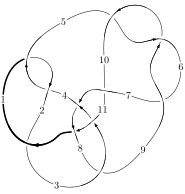
\includegraphics[width=112pt]{../../../GIT/diagram.site/Diagrams/png/318_11a_69.png}\\
\ \ \ A knot diagram\footnotemark}&
\allowdisplaybreaks
\textbf{Linearized knot diagam} \\
\cline{2-2}
 &
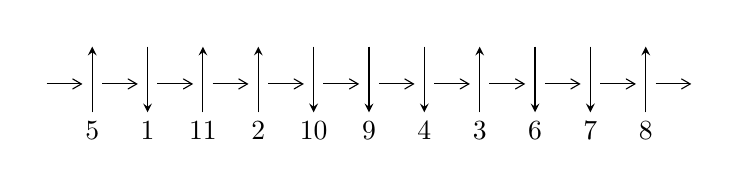
\begin{tikzpicture}[x=20pt, y=17pt]
	% nodes
	\node (C0) at (0, 0) {};
	\node (C1) at (1, 0) {};
	\node (C1U) at (1, +1) {};
	\node (C1D) at (1, -1) {5};

	\node (C2) at (2, 0) {};
	\node (C2U) at (2, +1) {};
	\node (C2D) at (2, -1) {1};

	\node (C3) at (3, 0) {};
	\node (C3U) at (3, +1) {};
	\node (C3D) at (3, -1) {11};

	\node (C4) at (4, 0) {};
	\node (C4U) at (4, +1) {};
	\node (C4D) at (4, -1) {2};

	\node (C5) at (5, 0) {};
	\node (C5U) at (5, +1) {};
	\node (C5D) at (5, -1) {10};

	\node (C6) at (6, 0) {};
	\node (C6U) at (6, +1) {};
	\node (C6D) at (6, -1) {9};

	\node (C7) at (7, 0) {};
	\node (C7U) at (7, +1) {};
	\node (C7D) at (7, -1) {4};

	\node (C8) at (8, 0) {};
	\node (C8U) at (8, +1) {};
	\node (C8D) at (8, -1) {3};

	\node (C9) at (9, 0) {};
	\node (C9U) at (9, +1) {};
	\node (C9D) at (9, -1) {6};

	\node (C10) at (10, 0) {};
	\node (C10U) at (10, +1) {};
	\node (C10D) at (10, -1) {7};

	\node (C11) at (11, 0) {};
	\node (C11U) at (11, +1) {};
	\node (C11D) at (11, -1) {8};
	\node (C12) at (12, 0) {};

	% arrows
	\draw[->,>={angle 60}]
	(C0) edge (C1) (C1) edge (C2) (C2) edge (C3) (C3) edge (C4) (C4) edge (C5) (C5) edge (C6) (C6) edge (C7) (C7) edge (C8) (C8) edge (C9) (C9) edge (C10) (C10) edge (C11) (C11) edge (C12) ;	\draw[->,>=stealth]
	(C1D) edge (C1U) (C2U) edge (C2D) (C3D) edge (C3U) (C4D) edge (C4U) (C5U) edge (C5D) (C6U) edge (C6D) (C7U) edge (C7D) (C8D) edge (C8U) (C9U) edge (C9D) (C10U) edge (C10D) (C11D) edge (C11U) ;
	\end{tikzpicture} \\
\hhline{~~} \\& 
\textbf{Solving Sequence} \\ \cline{2-2} 
 &
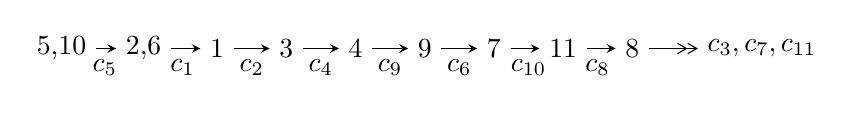
\begin{tikzpicture}[x=25pt, y=7pt]
	% node
	\node (A0) at (-1/8, 0) {5,10};
	\node (A1) at (17/16, 0) {2,6};
	\node (A2) at (17/8, 0) {1};
	\node (A3) at (25/8, 0) {3};
	\node (A4) at (33/8, 0) {4};
	\node (A5) at (41/8, 0) {9};
	\node (A6) at (49/8, 0) {7};
	\node (A7) at (57/8, 0) {11};
	\node (A8) at (65/8, 0) {8};
	\node (C1) at (1/2, -1) {$c_{5}$};
	\node (C2) at (13/8, -1) {$c_{1}$};
	\node (C3) at (21/8, -1) {$c_{2}$};
	\node (C4) at (29/8, -1) {$c_{4}$};
	\node (C5) at (37/8, -1) {$c_{9}$};
	\node (C6) at (45/8, -1) {$c_{6}$};
	\node (C7) at (53/8, -1) {$c_{10}$};
	\node (C8) at (61/8, -1) {$c_{8}$};
	\node (A9) at (10, 0) {$c_{3},c_{7},c_{11}$};

	% edge
	\draw[->,>=stealth]	
	(A0) edge (A1) (A1) edge (A2) (A2) edge (A3) (A3) edge (A4) (A4) edge (A5) (A5) edge (A6) (A6) edge (A7) (A7) edge (A8) ;
	\draw[->>,>={angle 60}]	
	(A8) edge (A9);
\end{tikzpicture} \\ 

\end{tabular} \\

\footnotetext{
The image of knot diagram is generated by the software ``\textbf{Draw programme}" developed by Andrew Bartholomew(\url{http://www.layer8.co.uk/maths/draw/index.htm\#Running-draw}), where we modified some parts for our purpose(\url{https://github.com/CATsTAILs/LinksPainter}).
}\phantom \\ \newline 
\centering \textbf{Ideals for irreducible components\footnotemark of $X_{\text{par}}$} 
 
\begin{align*}
I^u_{1}&=\langle 
1.93466\times10^{44} u^{69}+1.74032\times10^{45} u^{68}+\cdots+8.25681\times10^{45} b+7.83469\times10^{45},\\
\phantom{I^u_{1}}&\phantom{= \langle  }5.13127\times10^{45} u^{69}+8.43947\times10^{44} u^{68}+\cdots+8.25681\times10^{45} a-4.71677\times10^{45},\;u^{70}+u^{69}+\cdots+5 u+1\rangle \\
\\
\end{align*}
\raggedright * 1 irreducible components of $\dim_{\mathbb{C}}=0$, with total 70 representations.\\
\footnotetext{All coefficients of polynomials are rational numbers. But the coefficients are sometimes approximated in decimal forms when there is not enough margin.}
\newpage
\renewcommand{\arraystretch}{1}
\centering \section*{I. $I^u_{1}= \langle 1.93\times10^{44} u^{69}+1.74\times10^{45} u^{68}+\cdots+8.26\times10^{45} b+7.83\times10^{45},\;5.13\times10^{45} u^{69}+8.44\times10^{44} u^{68}+\cdots+8.26\times10^{45} a-4.72\times10^{45},\;u^{70}+u^{69}+\cdots+5 u+1 \rangle$}
\flushleft \textbf{(i) Arc colorings}\\
\begin{tabular}{m{7pt} m{180pt} m{7pt} m{180pt} }
\flushright $a_{5}=$&$\begin{pmatrix}1\\0\end{pmatrix}$ \\
\flushright $a_{10}=$&$\begin{pmatrix}0\\u\end{pmatrix}$ \\
\flushright $a_{2}=$&$\begin{pmatrix}-0.621458 u^{69}-0.102212 u^{68}+\cdots-1.03500 u+0.571258\\-0.0234310 u^{69}-0.210773 u^{68}+\cdots-5.77695 u-0.948876\end{pmatrix}$ \\
\flushright $a_{6}=$&$\begin{pmatrix}1\\u^2\end{pmatrix}$ \\
\flushright $a_{1}=$&$\begin{pmatrix}-0.598027 u^{69}+0.108561 u^{68}+\cdots+4.74196 u+1.52013\\-0.0234310 u^{69}-0.210773 u^{68}+\cdots-5.77695 u-0.948876\end{pmatrix}$ \\
\flushright $a_{3}=$&$\begin{pmatrix}-0.755347 u^{69}+0.563488 u^{68}+\cdots-11.1749 u-1.14377\\0.00374491 u^{69}-0.220825 u^{68}+\cdots-5.42897 u-1.96817\end{pmatrix}$ \\
\flushright $a_{4}=$&$\begin{pmatrix}-0.586927 u^{69}+0.648245 u^{68}+\cdots-11.4105 u-1.27713\\-0.0206773 u^{69}-0.191932 u^{68}+\cdots-5.40917 u-1.81465\end{pmatrix}$ \\
\flushright $a_{9}=$&$\begin{pmatrix}u\\u^3+u\end{pmatrix}$ \\
\flushright $a_{7}=$&$\begin{pmatrix}u^2+1\\u^4+2 u^2\end{pmatrix}$ \\
\flushright $a_{11}=$&$\begin{pmatrix}- u^5-2 u^3- u\\- u^7-3 u^5-2 u^3+u\end{pmatrix}$ \\
\flushright $a_{8}=$&$\begin{pmatrix}-0.196281 u^{69}+0.196656 u^{68}+\cdots-2.97884 u-0.704438\\-0.119642 u^{69}-0.282284 u^{68}+\cdots+2.93455 u+0.00852081\end{pmatrix}$\\ \flushright $a_{8}=$&$\begin{pmatrix}-0.196281 u^{69}+0.196656 u^{68}+\cdots-2.97884 u-0.704438\\-0.119642 u^{69}-0.282284 u^{68}+\cdots+2.93455 u+0.00852081\end{pmatrix}$\\&\end{tabular}
\flushleft \textbf{(ii) Obstruction class $= -1$}\\~\\
\flushleft \textbf{(iii) Cusp Shapes $= -3.55662 u^{69}-1.96540 u^{68}+\cdots+29.0576 u+10.9549$}\\~\\
\newpage\renewcommand{\arraystretch}{1}
\flushleft \textbf{(iv) u-Polynomials at the component}\newline \\
\begin{tabular}{m{50pt}|m{274pt}}
Crossings & \hspace{64pt}u-Polynomials at each crossing \\
\hline $$\begin{aligned}c_{1},c_{4}\end{aligned}$$&$\begin{aligned}
&u^{70}+u^{69}+\cdots+7 u+1
\end{aligned}$\\
\hline $$\begin{aligned}c_{2}\end{aligned}$$&$\begin{aligned}
&u^{70}+29 u^{69}+\cdots+7 u+1
\end{aligned}$\\
\hline $$\begin{aligned}c_{3}\end{aligned}$$&$\begin{aligned}
&u^{70}+7 u^{69}+\cdots+u+1
\end{aligned}$\\
\hline $$\begin{aligned}c_{5},c_{6},c_{9}\end{aligned}$$&$\begin{aligned}
&u^{70}- u^{69}+\cdots-5 u+1
\end{aligned}$\\
\hline $$\begin{aligned}c_{7}\end{aligned}$$&$\begin{aligned}
&u^{70}+3 u^{69}+\cdots-23 u+1
\end{aligned}$\\
\hline $$\begin{aligned}c_{8}\end{aligned}$$&$\begin{aligned}
&u^{70}+u^{69}+\cdots+49 u+4
\end{aligned}$\\
\hline $$\begin{aligned}c_{10}\end{aligned}$$&$\begin{aligned}
&u^{70}+u^{69}+\cdots-1887 u+578
\end{aligned}$\\
\hline $$\begin{aligned}c_{11}\end{aligned}$$&$\begin{aligned}
&u^{70}-5 u^{69}+\cdots- u+1
\end{aligned}$\\
\hline
\end{tabular}\\~\\
\newpage\renewcommand{\arraystretch}{1}
\flushleft \textbf{(v) Riley Polynomials at the component}\newline \\
\begin{tabular}{m{50pt}|m{274pt}}
Crossings & \hspace{64pt}Riley Polynomials at each crossing \\
\hline $$\begin{aligned}c_{1},c_{4}\end{aligned}$$&$\begin{aligned}
&y^{70}+29 y^{69}+\cdots+7 y+1
\end{aligned}$\\
\hline $$\begin{aligned}c_{2}\end{aligned}$$&$\begin{aligned}
&y^{70}+25 y^{69}+\cdots+347 y+1
\end{aligned}$\\
\hline $$\begin{aligned}c_{3}\end{aligned}$$&$\begin{aligned}
&y^{70}+5 y^{69}+\cdots+7 y+1
\end{aligned}$\\
\hline $$\begin{aligned}c_{5},c_{6},c_{9}\end{aligned}$$&$\begin{aligned}
&y^{70}+61 y^{69}+\cdots-5 y+1
\end{aligned}$\\
\hline $$\begin{aligned}c_{7}\end{aligned}$$&$\begin{aligned}
&y^{70}-71 y^{69}+\cdots-45 y+1
\end{aligned}$\\
\hline $$\begin{aligned}c_{8}\end{aligned}$$&$\begin{aligned}
&y^{70}-75 y^{69}+\cdots-401 y+16
\end{aligned}$\\
\hline $$\begin{aligned}c_{10}\end{aligned}$$&$\begin{aligned}
&y^{70}-15 y^{69}+\cdots-869601 y+334084
\end{aligned}$\\
\hline $$\begin{aligned}c_{11}\end{aligned}$$&$\begin{aligned}
&y^{70}-7 y^{69}+\cdots-5 y+1
\end{aligned}$\\
\hline
\end{tabular}\\~\\
\newpage\flushleft \textbf{(vi) Complex Volumes and Cusp Shapes}
$$\begin{array}{c|c|c}  
\text{Solutions to }I^u_{1}& \I (\text{vol} + \sqrt{-1}CS) & \text{Cusp shape}\\
 \hline 
\begin{aligned}
u &= -0.484335 + 0.875355 I \\
a &= -0.060674 + 0.946739 I \\
b &= -0.620167 + 1.091350 I\end{aligned}
 & \phantom{-}0.05172 - 8.00134 I & \phantom{-0.000000 } 0 \\ \hline\begin{aligned}
u &= -0.484335 - 0.875355 I \\
a &= -0.060674 - 0.946739 I \\
b &= -0.620167 - 1.091350 I\end{aligned}
 & \phantom{-}0.05172 + 8.00134 I & \phantom{-0.000000 } 0 \\ \hline\begin{aligned}
u &= \phantom{-}0.236828 + 1.056350 I \\
a &= \phantom{-}0.383136 - 0.264141 I \\
b &= -0.489406 - 0.250651 I\end{aligned}
 & \phantom{-}1.23691 - 2.50489 I & \phantom{-0.000000 } 0 \\ \hline\begin{aligned}
u &= \phantom{-}0.236828 - 1.056350 I \\
a &= \phantom{-}0.383136 + 0.264141 I \\
b &= -0.489406 + 0.250651 I\end{aligned}
 & \phantom{-}1.23691 + 2.50489 I & \phantom{-0.000000 } 0 \\ \hline\begin{aligned}
u &= \phantom{-}0.829379 + 0.365662 I \\
a &= \phantom{-}0.94611 + 1.69775 I \\
b &= -0.469428 + 0.973496 I\end{aligned}
 & -2.85780 - 3.99529 I & -10.44720 + 9.33363 I \\ \hline\begin{aligned}
u &= \phantom{-}0.829379 - 0.365662 I \\
a &= \phantom{-}0.94611 - 1.69775 I \\
b &= -0.469428 - 0.973496 I\end{aligned}
 & -2.85780 + 3.99529 I & -10.44720 - 9.33363 I \\ \hline\begin{aligned}
u &= \phantom{-}0.899262 + 0.112004 I \\
a &= -0.09567 - 1.68409 I \\
b &= -0.406148 - 0.936613 I\end{aligned}
 & -3.33093 + 1.52607 I & -13.07472 - 1.31899 I \\ \hline\begin{aligned}
u &= \phantom{-}0.899262 - 0.112004 I \\
a &= -0.09567 + 1.68409 I \\
b &= -0.406148 + 0.936613 I\end{aligned}
 & -3.33093 - 1.52607 I & -13.07472 + 1.31899 I \\ \hline\begin{aligned}
u &= -0.289959 + 1.067950 I \\
a &= \phantom{-}1.02846 - 1.50899 I \\
b &= -0.140513 - 1.175150 I\end{aligned}
 & -3.16104 - 0.50300 I & \phantom{-0.000000 } 0 \\ \hline\begin{aligned}
u &= -0.289959 - 1.067950 I \\
a &= \phantom{-}1.02846 + 1.50899 I \\
b &= -0.140513 + 1.175150 I\end{aligned}
 & -3.16104 + 0.50300 I & \phantom{-0.000000 } 0\\
 \hline 
 \end{array}$$\newpage$$\begin{array}{c|c|c}  
\text{Solutions to }I^u_{1}& \I (\text{vol} + \sqrt{-1}CS) & \text{Cusp shape}\\
 \hline 
\begin{aligned}
u &= -0.403491 + 0.782625 I \\
a &= \phantom{-}0.390557 - 0.716194 I \\
b &= -0.768228 - 0.457281 I\end{aligned}
 & \phantom{-}1.92693 - 2.73519 I & \phantom{-}2.12851 + 1.17713 I \\ \hline\begin{aligned}
u &= -0.403491 - 0.782625 I \\
a &= \phantom{-}0.390557 + 0.716194 I \\
b &= -0.768228 + 0.457281 I\end{aligned}
 & \phantom{-}1.92693 + 2.73519 I & \phantom{-}2.12851 - 1.17713 I \\ \hline\begin{aligned}
u &= \phantom{-}0.499100 + 1.027490 I \\
a &= \phantom{-}0.80149 + 1.34174 I \\
b &= -0.507327 + 1.004450 I\end{aligned}
 & -0.50648 - 6.46270 I & \phantom{-0.000000 } 0 \\ \hline\begin{aligned}
u &= \phantom{-}0.499100 - 1.027490 I \\
a &= \phantom{-}0.80149 - 1.34174 I \\
b &= -0.507327 - 1.004450 I\end{aligned}
 & -0.50648 + 6.46270 I & \phantom{-0.000000 } 0 \\ \hline\begin{aligned}
u &= -0.814672 + 0.264193 I \\
a &= \phantom{-}0.73755 - 2.31927 I \\
b &= -0.652177 - 1.126720 I\end{aligned}
 & -1.87843 + 12.59620 I & -3.11036 - 9.02697 I \\ \hline\begin{aligned}
u &= -0.814672 - 0.264193 I \\
a &= \phantom{-}0.73755 + 2.31927 I \\
b &= -0.652177 + 1.126720 I\end{aligned}
 & -1.87843 - 12.59620 I & -3.11036 + 9.02697 I \\ \hline\begin{aligned}
u &= -0.764380 + 0.264018 I \\
a &= -0.812441 - 0.044328 I \\
b &= -0.884444 + 0.447119 I\end{aligned}
 & \phantom{-}0.17592 + 6.93073 I & -0.67959 - 5.56176 I \\ \hline\begin{aligned}
u &= -0.764380 - 0.264018 I \\
a &= -0.812441 + 0.044328 I \\
b &= -0.884444 - 0.447119 I\end{aligned}
 & \phantom{-}0.17592 - 6.93073 I & -0.67959 + 5.56176 I \\ \hline\begin{aligned}
u &= \phantom{-}0.562477 + 0.578232 I \\
a &= \phantom{-}0.208519 - 0.713965 I \\
b &= -0.297139 - 0.882531 I\end{aligned}
 & -1.94107 - 0.75277 I & -7.49106 + 4.95501 I \\ \hline\begin{aligned}
u &= \phantom{-}0.562477 - 0.578232 I \\
a &= \phantom{-}0.208519 + 0.713965 I \\
b &= -0.297139 + 0.882531 I\end{aligned}
 & -1.94107 + 0.75277 I & -7.49106 - 4.95501 I\\
 \hline 
 \end{array}$$\newpage$$\begin{array}{c|c|c}  
\text{Solutions to }I^u_{1}& \I (\text{vol} + \sqrt{-1}CS) & \text{Cusp shape}\\
 \hline 
\begin{aligned}
u &= -0.745456 + 0.148738 I \\
a &= -0.36458 + 2.64857 I \\
b &= -0.050089 + 1.257290 I\end{aligned}
 & -5.92974 + 4.34707 I & -7.96325 - 5.56332 I \\ \hline\begin{aligned}
u &= -0.745456 - 0.148738 I \\
a &= -0.36458 - 2.64857 I \\
b &= -0.050089 - 1.257290 I\end{aligned}
 & -5.92974 - 4.34707 I & -7.96325 + 5.56332 I \\ \hline\begin{aligned}
u &= -0.107903 + 1.245720 I \\
a &= \phantom{-}0.523629 - 1.003470 I \\
b &= \phantom{-}0.416221 - 1.189180 I\end{aligned}
 & \phantom{-}1.99705 - 2.44523 I & \phantom{-0.000000 } 0 \\ \hline\begin{aligned}
u &= -0.107903 - 1.245720 I \\
a &= \phantom{-}0.523629 + 1.003470 I \\
b &= \phantom{-}0.416221 + 1.189180 I\end{aligned}
 & \phantom{-}1.99705 + 2.44523 I & \phantom{-0.000000 } 0 \\ \hline\begin{aligned}
u &= \phantom{-}0.200108 + 1.261720 I \\
a &= \phantom{-}0.32731 + 2.79217 I \\
b &= \phantom{-}0.401964 + 0.917807 I\end{aligned}
 & \phantom{-}2.39518 - 0.54119 I & \phantom{-0.000000 } 0 \\ \hline\begin{aligned}
u &= \phantom{-}0.200108 - 1.261720 I \\
a &= \phantom{-}0.32731 - 2.79217 I \\
b &= \phantom{-}0.401964 - 0.917807 I\end{aligned}
 & \phantom{-}2.39518 + 0.54119 I & \phantom{-0.000000 } 0 \\ \hline\begin{aligned}
u &= \phantom{-}0.368590 + 1.279980 I \\
a &= -0.036929 - 0.922221 I \\
b &= -0.254902 - 0.847557 I\end{aligned}
 & \phantom{-}0.95320 - 3.02207 I & \phantom{-0.000000 } 0 \\ \hline\begin{aligned}
u &= \phantom{-}0.368590 - 1.279980 I \\
a &= -0.036929 + 0.922221 I \\
b &= -0.254902 + 0.847557 I\end{aligned}
 & \phantom{-}0.95320 + 3.02207 I & \phantom{-0.000000 } 0 \\ \hline\begin{aligned}
u &= \phantom{-}0.193666 + 1.332510 I \\
a &= -0.68225 - 2.26640 I \\
b &= \phantom{-}0.541955 + 0.776960 I\end{aligned}
 & \phantom{-}3.56607 - 0.95896 I & \phantom{-0.000000 } 0 \\ \hline\begin{aligned}
u &= \phantom{-}0.193666 - 1.332510 I \\
a &= -0.68225 + 2.26640 I \\
b &= \phantom{-}0.541955 - 0.776960 I\end{aligned}
 & \phantom{-}3.56607 + 0.95896 I & \phantom{-0.000000 } 0\\
 \hline 
 \end{array}$$\newpage$$\begin{array}{c|c|c}  
\text{Solutions to }I^u_{1}& \I (\text{vol} + \sqrt{-1}CS) & \text{Cusp shape}\\
 \hline 
\begin{aligned}
u &= -0.150263 + 1.338740 I \\
a &= -0.223687 + 0.346604 I \\
b &= \phantom{-}0.838536 - 0.993294 I\end{aligned}
 & \phantom{-}5.26003 - 1.16982 I & \phantom{-0.000000 } 0 \\ \hline\begin{aligned}
u &= -0.150263 - 1.338740 I \\
a &= -0.223687 - 0.346604 I \\
b &= \phantom{-}0.838536 + 0.993294 I\end{aligned}
 & \phantom{-}5.26003 + 1.16982 I & \phantom{-0.000000 } 0 \\ \hline\begin{aligned}
u &= \phantom{-}0.231094 + 1.328390 I \\
a &= -3.66836 - 1.80527 I \\
b &= \phantom{-}0.536274 - 0.919865 I\end{aligned}
 & \phantom{-}3.11019 - 5.29914 I & \phantom{-0.000000 } 0 \\ \hline\begin{aligned}
u &= \phantom{-}0.231094 - 1.328390 I \\
a &= -3.66836 + 1.80527 I \\
b &= \phantom{-}0.536274 + 0.919865 I\end{aligned}
 & \phantom{-}3.11019 + 5.29914 I & \phantom{-0.000000 } 0 \\ \hline\begin{aligned}
u &= \phantom{-}0.611770 + 0.194791 I \\
a &= \phantom{-}0.407403 + 0.167127 I \\
b &= -0.224664 - 0.169997 I\end{aligned}
 & -1.37636 - 0.69918 I & -5.13733 + 2.33652 I \\ \hline\begin{aligned}
u &= \phantom{-}0.611770 - 0.194791 I \\
a &= \phantom{-}0.407403 - 0.167127 I \\
b &= -0.224664 + 0.169997 I\end{aligned}
 & -1.37636 + 0.69918 I & -5.13733 - 2.33652 I \\ \hline\begin{aligned}
u &= -0.613468 + 0.166353 I \\
a &= -0.44642 + 2.95844 I \\
b &= \phantom{-}0.616639 + 1.172650 I\end{aligned}
 & -0.93135 + 4.88535 I & -2.28013 - 10.40687 I \\ \hline\begin{aligned}
u &= -0.613468 - 0.166353 I \\
a &= -0.44642 - 2.95844 I \\
b &= \phantom{-}0.616639 - 1.172650 I\end{aligned}
 & -0.93135 - 4.88535 I & -2.28013 + 10.40687 I \\ \hline\begin{aligned}
u &= \phantom{-}0.200597 + 1.358150 I \\
a &= \phantom{-}0.286571 + 0.255300 I \\
b &= \phantom{-}0.250675 - 0.338013 I\end{aligned}
 & \phantom{-}3.63488 - 3.48634 I & \phantom{-0.000000 } 0 \\ \hline\begin{aligned}
u &= \phantom{-}0.200597 - 1.358150 I \\
a &= \phantom{-}0.286571 - 0.255300 I \\
b &= \phantom{-}0.250675 + 0.338013 I\end{aligned}
 & \phantom{-}3.63488 + 3.48634 I & \phantom{-0.000000 } 0\\
 \hline 
 \end{array}$$\newpage$$\begin{array}{c|c|c}  
\text{Solutions to }I^u_{1}& \I (\text{vol} + \sqrt{-1}CS) & \text{Cusp shape}\\
 \hline 
\begin{aligned}
u &= -0.183760 + 1.364120 I \\
a &= -0.072592 + 0.787390 I \\
b &= \phantom{-}1.003970 - 0.281861 I\end{aligned}
 & \phantom{-}6.67319 + 1.90375 I & \phantom{-0.000000 } 0 \\ \hline\begin{aligned}
u &= -0.183760 - 1.364120 I \\
a &= -0.072592 - 0.787390 I \\
b &= \phantom{-}1.003970 + 0.281861 I\end{aligned}
 & \phantom{-}6.67319 - 1.90375 I & \phantom{-0.000000 } 0 \\ \hline\begin{aligned}
u &= -0.247821 + 1.358540 I \\
a &= -1.60160 + 1.37832 I \\
b &= \phantom{-}0.693479 + 1.215560 I\end{aligned}
 & \phantom{-}3.90043 + 8.04691 I & \phantom{-0.000000 } 0 \\ \hline\begin{aligned}
u &= -0.247821 - 1.358540 I \\
a &= -1.60160 - 1.37832 I \\
b &= \phantom{-}0.693479 - 1.215560 I\end{aligned}
 & \phantom{-}3.90043 - 8.04691 I & \phantom{-0.000000 } 0 \\ \hline\begin{aligned}
u &= -0.212109 + 1.366200 I \\
a &= -0.941802 + 0.648116 I \\
b &= \phantom{-}1.001640 + 0.651261 I\end{aligned}
 & \phantom{-}6.29345 + 5.42481 I & \phantom{-0.000000 } 0 \\ \hline\begin{aligned}
u &= -0.212109 - 1.366200 I \\
a &= -0.941802 - 0.648116 I \\
b &= \phantom{-}1.001640 - 0.651261 I\end{aligned}
 & \phantom{-}6.29345 - 5.42481 I & \phantom{-0.000000 } 0 \\ \hline\begin{aligned}
u &= -0.303558 + 1.351170 I \\
a &= -0.92726 + 1.21935 I \\
b &= \phantom{-}0.006202 + 1.312430 I\end{aligned}
 & -1.19896 + 8.13596 I & \phantom{-0.000000 } 0 \\ \hline\begin{aligned}
u &= -0.303558 - 1.351170 I \\
a &= -0.92726 - 1.21935 I \\
b &= \phantom{-}0.006202 - 1.312430 I\end{aligned}
 & -1.19896 - 8.13596 I & \phantom{-0.000000 } 0 \\ \hline\begin{aligned}
u &= \phantom{-}0.594534 + 0.061490 I \\
a &= -2.14747 - 5.13430 I \\
b &= \phantom{-}0.485312 - 0.908136 I\end{aligned}
 & -1.29895 - 2.30609 I & \phantom{-}11.5630 - 16.8929 I \\ \hline\begin{aligned}
u &= \phantom{-}0.594534 - 0.061490 I \\
a &= -2.14747 + 5.13430 I \\
b &= \phantom{-}0.485312 + 0.908136 I\end{aligned}
 & -1.29895 + 2.30609 I & \phantom{-}11.5630 + 16.8929 I\\
 \hline 
 \end{array}$$\newpage$$\begin{array}{c|c|c}  
\text{Solutions to }I^u_{1}& \I (\text{vol} + \sqrt{-1}CS) & \text{Cusp shape}\\
 \hline 
\begin{aligned}
u &= -0.30882 + 1.41041 I \\
a &= -0.018285 - 0.748543 I \\
b &= -0.938125 + 0.475226 I\end{aligned}
 & \phantom{-}5.50503 + 10.82290 I & \phantom{-0.000000 } 0 \\ \hline\begin{aligned}
u &= -0.30882 - 1.41041 I \\
a &= -0.018285 + 0.748543 I \\
b &= -0.938125 - 0.475226 I\end{aligned}
 & \phantom{-}5.50503 - 10.82290 I & \phantom{-0.000000 } 0 \\ \hline\begin{aligned}
u &= -0.33175 + 1.41736 I \\
a &= \phantom{-}1.66811 - 1.38164 I \\
b &= -0.680160 - 1.138340 I\end{aligned}
 & \phantom{-}3.4715 + 16.7403 I & \phantom{-0.000000 } 0 \\ \hline\begin{aligned}
u &= -0.33175 - 1.41736 I \\
a &= \phantom{-}1.66811 + 1.38164 I \\
b &= -0.680160 + 1.138340 I\end{aligned}
 & \phantom{-}3.4715 - 16.7403 I & \phantom{-0.000000 } 0 \\ \hline\begin{aligned}
u &= \phantom{-}0.26824 + 1.43648 I \\
a &= \phantom{-}0.320427 + 0.345844 I \\
b &= -0.519294 - 0.588568 I\end{aligned}
 & \phantom{-}4.08495 - 3.81337 I & \phantom{-0.000000 } 0 \\ \hline\begin{aligned}
u &= \phantom{-}0.26824 - 1.43648 I \\
a &= \phantom{-}0.320427 - 0.345844 I \\
b &= -0.519294 + 0.588568 I\end{aligned}
 & \phantom{-}4.08495 + 3.81337 I & \phantom{-0.000000 } 0 \\ \hline\begin{aligned}
u &= -0.487601 + 0.208801 I \\
a &= \phantom{-}0.30455 + 1.43000 I \\
b &= \phantom{-}0.833768 + 0.669179 I\end{aligned}
 & \phantom{-}1.32084 + 2.75218 I & \phantom{-}4.00267 - 8.42337 I \\ \hline\begin{aligned}
u &= -0.487601 - 0.208801 I \\
a &= \phantom{-}0.30455 - 1.43000 I \\
b &= \phantom{-}0.833768 - 0.669179 I\end{aligned}
 & \phantom{-}1.32084 - 2.75218 I & \phantom{-}4.00267 + 8.42337 I \\ \hline\begin{aligned}
u &= -0.04696 + 1.47919 I \\
a &= \phantom{-}1.013550 - 0.079452 I \\
b &= -0.776577 - 0.650017 I\end{aligned}
 & \phantom{-}9.19605 - 1.61168 I & \phantom{-0.000000 } 0 \\ \hline\begin{aligned}
u &= -0.04696 - 1.47919 I \\
a &= \phantom{-}1.013550 + 0.079452 I \\
b &= -0.776577 + 0.650017 I\end{aligned}
 & \phantom{-}9.19605 + 1.61168 I & \phantom{-0.000000 } 0\\
 \hline 
 \end{array}$$\newpage$$\begin{array}{c|c|c}  
\text{Solutions to }I^u_{1}& \I (\text{vol} + \sqrt{-1}CS) & \text{Cusp shape}\\
 \hline 
\begin{aligned}
u &= \phantom{-}0.34186 + 1.45082 I \\
a &= \phantom{-}1.47158 + 1.05054 I \\
b &= -0.558838 + 0.987517 I\end{aligned}
 & \phantom{-}2.91206 - 8.27553 I & \phantom{-0.000000 } 0 \\ \hline\begin{aligned}
u &= \phantom{-}0.34186 - 1.45082 I \\
a &= \phantom{-}1.47158 - 1.05054 I \\
b &= -0.558838 - 0.987517 I\end{aligned}
 & \phantom{-}2.91206 + 8.27553 I & \phantom{-0.000000 } 0 \\ \hline\begin{aligned}
u &= -0.00295 + 1.51219 I \\
a &= \phantom{-}0.927152 + 0.098522 I \\
b &= -0.667838 + 0.997816 I\end{aligned}
 & \phantom{-}8.13804 - 7.06461 I & \phantom{-0.000000 } 0 \\ \hline\begin{aligned}
u &= -0.00295 - 1.51219 I \\
a &= \phantom{-}0.927152 - 0.098522 I \\
b &= -0.667838 - 0.997816 I\end{aligned}
 & \phantom{-}8.13804 + 7.06461 I & \phantom{-0.000000 } 0 \\ \hline\begin{aligned}
u &= \phantom{-}0.473311 + 0.093934 I \\
a &= \phantom{-}2.06318 - 1.63899 I \\
b &= \phantom{-}0.437497 + 0.816872 I\end{aligned}
 & -0.93813 + 1.54075 I & -3.94589 - 11.49495 I \\ \hline\begin{aligned}
u &= \phantom{-}0.473311 - 0.093934 I \\
a &= \phantom{-}2.06318 + 1.63899 I \\
b &= \phantom{-}0.437497 - 0.816872 I\end{aligned}
 & -0.93813 - 1.54075 I & -3.94589 + 11.49495 I \\ \hline\begin{aligned}
u &= -0.380898 + 0.262790 I \\
a &= \phantom{-}1.44857 + 0.52153 I \\
b &= \phantom{-}0.728444 - 0.317658 I\end{aligned}
 & \phantom{-}1.64058 - 0.33786 I & \phantom{-}6.07692 - 1.73353 I \\ \hline\begin{aligned}
u &= -0.380898 - 0.262790 I \\
a &= \phantom{-}1.44857 - 0.52153 I \\
b &= \phantom{-}0.728444 + 0.317658 I\end{aligned}
 & \phantom{-}1.64058 + 0.33786 I & \phantom{-}6.07692 + 1.73353 I \\ \hline\begin{aligned}
u &= -0.130656 + 0.280023 I \\
a &= \phantom{-}1.342180 - 0.108395 I \\
b &= \phantom{-}0.612892 - 0.951335 I\end{aligned}
 & \phantom{-}0.54295 - 2.64582 I & \phantom{-}2.44579 + 0.83594 I \\ \hline\begin{aligned}
u &= -0.130656 - 0.280023 I \\
a &= \phantom{-}1.342180 + 0.108395 I \\
b &= \phantom{-}0.612892 + 0.951335 I\end{aligned}
 & \phantom{-}0.54295 + 2.64582 I & \phantom{-}2.44579 - 0.83594 I\\
 \hline 
 \end{array}$$\newpage
\newpage\renewcommand{\arraystretch}{1}
\centering \section*{ II. u-Polynomials}
\begin{tabular}{m{50pt}|m{274pt}}
Crossings & \hspace{64pt}u-Polynomials at each crossing \\
\hline $$\begin{aligned}c_{1},c_{4}\end{aligned}$$&$\begin{aligned}
&u^{70}+u^{69}+\cdots+7 u+1
\end{aligned}$\\
\hline $$\begin{aligned}c_{2}\end{aligned}$$&$\begin{aligned}
&u^{70}+29 u^{69}+\cdots+7 u+1
\end{aligned}$\\
\hline $$\begin{aligned}c_{3}\end{aligned}$$&$\begin{aligned}
&u^{70}+7 u^{69}+\cdots+u+1
\end{aligned}$\\
\hline $$\begin{aligned}c_{5},c_{6},c_{9}\end{aligned}$$&$\begin{aligned}
&u^{70}- u^{69}+\cdots-5 u+1
\end{aligned}$\\
\hline $$\begin{aligned}c_{7}\end{aligned}$$&$\begin{aligned}
&u^{70}+3 u^{69}+\cdots-23 u+1
\end{aligned}$\\
\hline $$\begin{aligned}c_{8}\end{aligned}$$&$\begin{aligned}
&u^{70}+u^{69}+\cdots+49 u+4
\end{aligned}$\\
\hline $$\begin{aligned}c_{10}\end{aligned}$$&$\begin{aligned}
&u^{70}+u^{69}+\cdots-1887 u+578
\end{aligned}$\\
\hline $$\begin{aligned}c_{11}\end{aligned}$$&$\begin{aligned}
&u^{70}-5 u^{69}+\cdots- u+1
\end{aligned}$\\
\hline
\end{tabular}\newpage\renewcommand{\arraystretch}{1}
\centering \section*{ III. Riley Polynomials}
\begin{tabular}{m{50pt}|m{274pt}}
Crossings & \hspace{64pt}Riley Polynomials at each crossing \\
\hline $$\begin{aligned}c_{1},c_{4}\end{aligned}$$&$\begin{aligned}
&y^{70}+29 y^{69}+\cdots+7 y+1
\end{aligned}$\\
\hline $$\begin{aligned}c_{2}\end{aligned}$$&$\begin{aligned}
&y^{70}+25 y^{69}+\cdots+347 y+1
\end{aligned}$\\
\hline $$\begin{aligned}c_{3}\end{aligned}$$&$\begin{aligned}
&y^{70}+5 y^{69}+\cdots+7 y+1
\end{aligned}$\\
\hline $$\begin{aligned}c_{5},c_{6},c_{9}\end{aligned}$$&$\begin{aligned}
&y^{70}+61 y^{69}+\cdots-5 y+1
\end{aligned}$\\
\hline $$\begin{aligned}c_{7}\end{aligned}$$&$\begin{aligned}
&y^{70}-71 y^{69}+\cdots-45 y+1
\end{aligned}$\\
\hline $$\begin{aligned}c_{8}\end{aligned}$$&$\begin{aligned}
&y^{70}-75 y^{69}+\cdots-401 y+16
\end{aligned}$\\
\hline $$\begin{aligned}c_{10}\end{aligned}$$&$\begin{aligned}
&y^{70}-15 y^{69}+\cdots-869601 y+334084
\end{aligned}$\\
\hline $$\begin{aligned}c_{11}\end{aligned}$$&$\begin{aligned}
&y^{70}-7 y^{69}+\cdots-5 y+1
\end{aligned}$\\
\hline
\end{tabular}
\vskip 2pc
\end{document}